%%%%%%%%%%%%%%%%%%%%%%%%%%%%%%%%%%%%%%%%%
% Programming/Coding Assignment
% LaTeX Template
%
% This template has been downloaded from:
% http://www.latextemplates.com
%
% Original author:
% Ted Pavlic (http://www.tedpavlic.com)
%
% Note:
% The \lipsum[#] commands throughout this template generate dummy text
% to fill the template out. These commands should all be removed when 
% writing assignment content.
%
% This template uses a Perl script as an example snippet of code, most other
% languages are also usable. Configure them in the "CODE INCLUSION 
% CONFIGURATION" section.
%
%%%%%%%%%%%%%%%%%%%%%%%%%%%%%%%%%%%%%%%%%

%----------------------------------------------------------------------------------------
%	PACKAGES AND OTHER DOCUMENT CONFIGURATIONS
%----------------------------------------------------------------------------------------

\documentclass{article}

\usepackage{fancyhdr} % Required for custom headers
\usepackage{lastpage} % Required to determine the last page for the footer
\usepackage{extramarks} % Required for headers and footers
\usepackage[usenames,dvipsnames]{color} % Required for custom colors
\usepackage{graphicx} % Required to insert images
\usepackage{listings} % Required for insertion of code
\usepackage{courier} % Required for the courier font
\usepackage{multirow}
\usepackage{hyperref}


% Margins
\topmargin=-0.45in
\evensidemargin=0in
\oddsidemargin=0in
\textwidth=6.5in
\textheight=9.0in
\headsep=0.25in

\linespread{1.1} % Line spacing

%----------------------------------------------------------------------------------------
%	CODE INCLUSION CONFIGURATION
%----------------------------------------------------------------------------------------

\definecolor{MyDarkGreen}{rgb}{0.0,0.4,0.0} % This is the color used for comments
\lstloadlanguages{c} % Load Perl syntax for listings, for a list of other languages supported see: ftp://ftp.tex.ac.uk/tex-archive/macros/latex/contrib/listings/listings.pdf
\lstset{language=[sharp]c, % Use Perl in this example
        frame=single, % Single frame around code
        basicstyle=\small\ttfamily, % Use small true type font
        keywordstyle=[1]\color{Blue}\bf, % Perl functions bold and blue
        keywordstyle=[2]\color{Purple}, % Perl function arguments purple
        keywordstyle=[3]\color{Blue}\underbar, % Custom functions underlined and blue
        identifierstyle=, % Nothing special about identifiers                                         
        commentstyle=\usefont{T1}{pcr}{m}{sl}\color{MyDarkGreen}\small, % Comments small dark green courier font
        stringstyle=\color{Purple}, % Strings are purple
        showstringspaces=false, % Don't put marks in string spaces
        tabsize=5, % 5 spaces per tab
        %
        % Put standard Perl functions not included in the default language here
        morekeywords={rand},
        %
        % Put Perl function parameters here
        morekeywords=[2]{on, off, interp},
        %
        % Put user defined functions here
        morekeywords=[3]{test},
       	%
        morecomment=[l][\color{Blue}]{...}, % Line continuation (...) like blue comment
        numbers=left, % Line numbers on left
        firstnumber=1, % Line numbers start with line 1
        numberstyle=\tiny\color{Blue}, % Line numbers are blue and small
        stepnumber=5 % Line numbers go in steps of 5
}

\newcommand{\horrule}[1]{\rule{\linewidth}{#1}}

% Creates a new command to include a perl script, the first parameter is the filename of the script (without .pl), the second parameter is the caption
\newcommand{\perlscript}[2]{
\begin{itemize}
\item[]\lstinputlisting[caption=#2,label=#1]{#1.cs}
\end{itemize}
}

\begin{document}

\begin{tabular}{l l}
\multirow{5}{*}{\includegraphics[width=2cm]{../../Recursos/logo.png}} & Universidad del Istmo de Guatemala \\
 & Facultad de Ingenieria \\
 & Ing. en Sistemas \\
 & Informatica 2 \\
 & Prof. Ernesto Rodriguez - \href{mailto:erodriguez@unis.edu.gt}{erodriguez@unis.edu.gt} \\
\end{tabular}
\\\\\\

\begin{center}
        \horrule{0.5pt}
        \huge{Hoja de trabajo \#8} \\
        \large{Fecha de entrega: 27 de Abril, 2018 - 11:59pm} \\
        \horrule{1pt}
\end{center}
\emph{Instrucciones: Realizar cada uno de los ejercicios siguiendo sus respectivas
instrucciones. El trabajo debe ser entregado a traves de Github, en su repositorio del curso, colocado en una carpeta llamada ``Hoja de trabajo 8''.
Al menos que la pregunta indique diferente, todas las respuestas a preguntas escritas deben presentarse en
un documento formato pdf, el cual haya sido generado mediante Latex. Los ejercicios de programaci\'on deben ser colocados en una carpeta
llamada ``Programas", la cual debe colocarse dentro de la carpeta correspondiente a esta hoja de trabajo.}

\section*{Iniciaci\'on}

Crear una soluci\'on llamada \emph{ParseTree}. Dentro de esta soluci\'on crear:
\begin{itemize}
        \item{un proyecto llamado \emph{ParseTree} de tipo console}
        \item{un proyecto llamado \emph{ParseTreeTests} de tipo xunit}
\end{itemize}

\section*{Parse tree (50\%)}
Un \emph{parse tree} o arbol de parseo es un arbol (en este caso un arbol binario) que corresponde a una
representaci\'on de todas las partes de un lenguaje. Consideremos el lenguaje de la aritmetica, el
cual contiene sumas ($+$) y multiplicaciones ($*$), podemos construir la expresi\'on $1+3*2+8$. Recordemos
que el orden en que se deben realizar las operaciones (seg\'un las reglas de procedencia de la aritmentica)
es el siguiente: ``$(1+(3*2))+8$''. A partir de este orden, podemos construir un arbol para representar dicha
operaci\'on y orden. El arbol seria el siguiente:
\\
\begin{center}
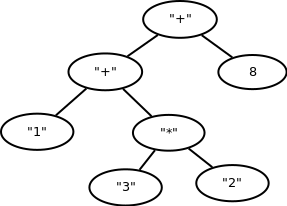
\includegraphics[width=10cm]{pTree.png}
\end{center}
Este arbol es facil construir recursivamente a partir de una expresi\'on matematica
como ``$1+3*2+8$''. Por simplicidad, se consideraran dos recorridos al arbol: (1)
expandir las sumas y (2) expandir las multiplicaciones. Consideremos de primero la
primera pasada. Se comienza con la expresi\'on entera colocada en un arbol con un
solo nodo (es un arbol que contiene \texttt{strings}):
\\
\begin{center}
        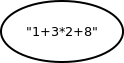
\includegraphics[width=3cm]{1ptree.png}
\end{center}
Luego se selecciona la suma de \emph{menor} procedencia (en otras palabras, la suma
m\'as a la derecha) y se divide la operaci\'on en ese punto. Por lo cual, a partir
de la operaci\'on  ``$1+3*2+8$'', obtenemos ``$1+3*2$'', ``$+$'' y ``$8$''. Luego
modificamos el nodo actual de tal forma que la operaci\'on queda en el nodo central
y las sub-operaciones a la derecha e izquierda quedan como nodos hijos. El arbol
ahora se ve asi:
\\
\begin{center}
        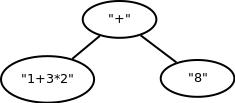
\includegraphics[width=6cm]{3ptree.png}
\end{center}
Luego, se ejecuta esta operaci\'on recursivamente en cada uno de los nodos nuevos.
Tomar en cuenta que al llegar a un nodo ``final'', como ``$8$'', este nodo ya no
se dividira en m\'as nodos debido a que no tiene una suma. Esto indica que la
recursi\'on debe parar ya que no hay m\'as nodos que expandir.
\\\\
Luego de haber expandido las sumas del arbol, se puede utilizar el mismo metodo
para expandir las multiplicaciones del arbol aplicando dicha operaci\'on en
cada uno de los nodos del arbol nuevo.
\\\\
\emph{Tarea:} 
\begin{enumerate}
        \item{Crear una clase llamada ``ParseTree'' que hereda de la clase
        ``BinaryTree'' especializando su tipo generico a \texttt{string}}
        \item{definir los metodos ``ExpandirSumas'', ``ExpandirMultiplicaciones'' y
        ``Expandir'' en la clase ``ParseTree'' que expandan los
        nodos de dicho arbol como se menciono anteriormente. El metodo ``Expandir'' simplemente
        aplica ``ExpandirSumas'' seguido de ``ExpandirMultiplicaciones''. Si lo desea, puede
        implementar toda la expansi\'on en un solo metodo.}
\end{enumerate}

\section*{Metodo \emph{Evaluar} (30\%)}
Luego de construir un arbol de parseo, es facil calcular cual seria el resultado
de la operaci\'on expresada por el arbol de parseo utilizando la funci\'on
\emph{Reduce}. Como recordatorio, \emph{Reduce} toma dos parametros: (1) una
funci\'on que indica como combinar el valor acutal del arbol con el derecho
y el izquierdo (funci\'on conocida como \emph{reducer}) (2) el valor que se
le pasara al \emph{reducer} en caso que el lado derecho o izquierdo sea nulo.
\\\\
Para calcular el resultado, se definira un \emph{reducer} que lleva a cabo
el trabajo. Como primer paso, definir un metodo en la clase ``ParseTree''
llamado ``ReducerAritmetico'' con tipo ``$\mathtt{ReducerAritmetico}
\ :\ \mathtt{int}\otimes\mathtt{int}\otimes\mathtt{string}\rightarrow\mathtt{int}$''.
Este metodo debe hacer lo siguiente:
\begin{enumerate}
        \item{Si el tercer parametro (el valor) es ``$+$'', retornar: izquierdo + derecho}
        \item{Si el tercer parametro (el valor) es ``$*$'', retornar: izquierdo * derecho}
        \item{De lo contrario, convertir el valor a entero utilizando la funcion \emph{Parse}
        de la clase \emph{int}: \texttt{int.Parse(valor)}. Retornar dicho valor.}
\end{enumerate}
A partir de esto, definir el metodo evaluar, el cual simplemente debe llamar
al metodo \emph{Reduce} utilizando cero (0) como valor inicial y ``ReducerAritmetico''
como su \emph{reducer} y retornar dicho valor.

\section*{Unit tests (20\%)}
En el proyecto ``ParseTreeTests'', definir un unit test que verifique que
un arbol de parseo inicializado con una expresi\'on aritmetica arbitraria,
puede evaluarla correctamente llamando primero al metodo ``Expandir'' para obtener
el parse tree correspondiente y luego llamando al metodo ``Evaluar''.

\end{document}